\documentclass[a3paper]{scrartcl}
\usepackage{fontawesome}
\usepackage{tikz}
\usepackage{url}
\usepackage{fullpage}
\usetikzlibrary{fit,positioning,arrows.meta,decorations.pathreplacing,calc}
\usepackage[outline]{contour}

\newcounter{protostep}[figure]
\renewcommand{\theprotostep}{\arabic{protostep}}
\def\protostep#1{\resizebox{!}{0.8\baselineskip}{\begin{tikzpicture}[baseline={([yshift=-0.5pt]O.base)}] \node (O) [sharp corners,fill=blue,inner sep=1ex]{\color{white}\textbf{\refstepcounter{protostep}\theprotostep\label{protostep:#1}}};\end{tikzpicture}}}
\def\refprotostep#1{\resizebox{!}{0.6\baselineskip}{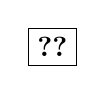
\begin{tikzpicture}[baseline={([yshift=-1.5pt]O.base)}] \node (O) [draw,sharp corners]{\ref{protostep:#1}};\end{tikzpicture}}}


\begin{document}
\section*{The Unicorn Protocol}
Figure~\ref{fig:unicorn} shows the unicorn protocol, which for now
serves as the documentation of the Annex language.
Step~\refprotostep{unicorn:some-request} is just as fictional as
Step~\refprotostep{unicorn:some-response}. We can refer to whole
groups of steps as well (\refprotostep{unicorn:condensed}).

\begin{figure}[h!]
  \centering  
  \input{demo.yml.tex}
  \caption{The Unicorn protocol, showing off some features of Annex.
    The protocol flow, all names, messages, and URLs portrayed in this
    chart are fictitious. No identification with actual protocols (in
    production or deprecated), deployments, and products is intended
    or should be inferred. No unicorns were harmed in the making of
    this protocol diagram.}
  \label{fig:unicorn}
\end{figure}
\end{document}